\section{Transport Layer}

\subsection{Transport-layer services}

\key{Internet transport-layer protocols}
\begin{itemize}
  \item Reliable, in-order delivery (TCP)
    \begin{itemize}
      \item congestion control
      \item flow control
      \item connection setup
    \end{itemize}

  \item Unreliable, unordered delivery (UDP)\\
    No-frills extension of ``best-effort'' IP
\end{itemize}

\subsection{Principles of reliable data transfer}

\key{Go-Back-N} Maximum window size is $N-1$
\begin{figure}[H]
  \centering
  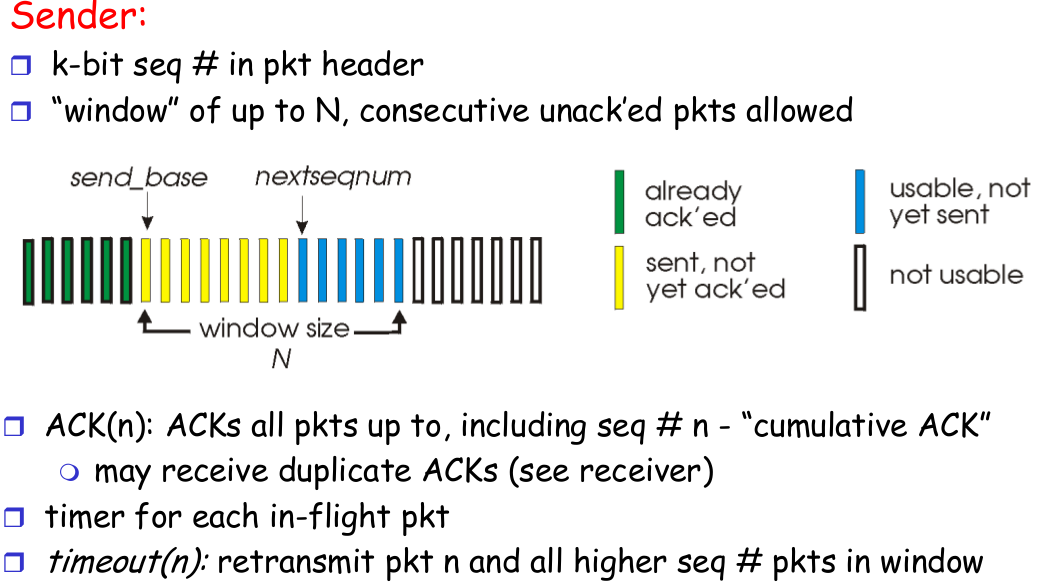
\includegraphics[width=0.48\textwidth]{gbn}
  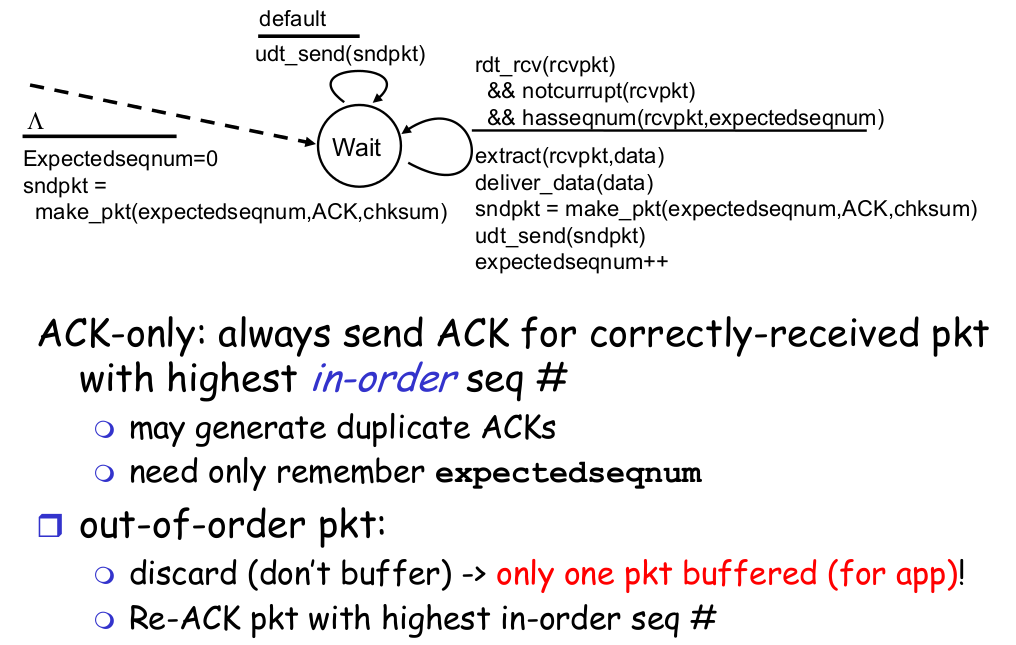
\includegraphics[width=0.48\textwidth]{gbn2}
\end{figure}

\key{Selective Repeat} Maximum window size is $N/2$
\begin{figure}[H]
  \centering
  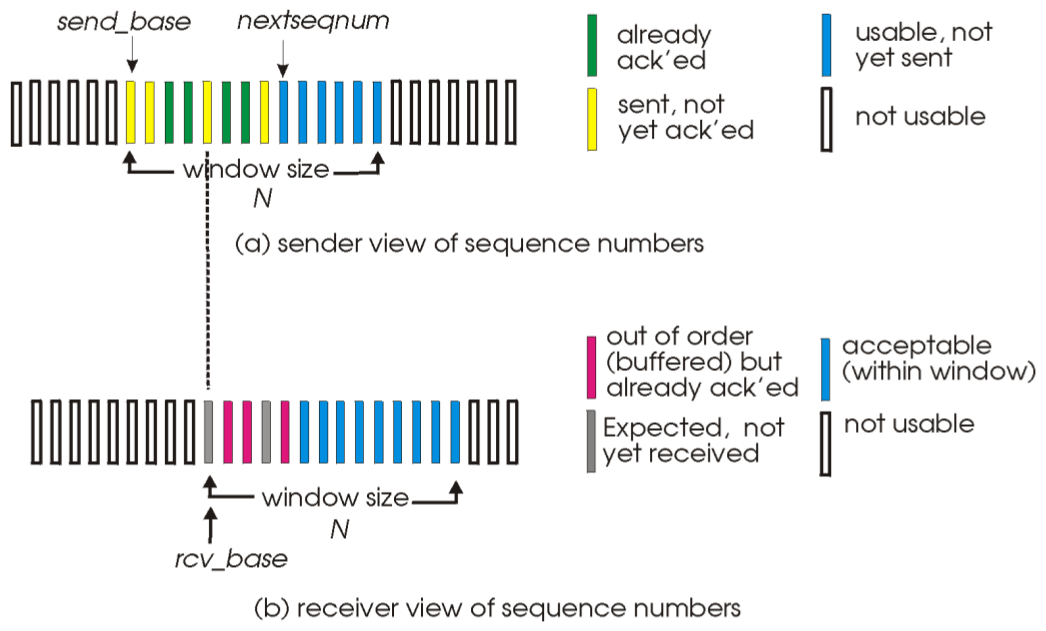
\includegraphics[width=0.48\textwidth]{sr2}
  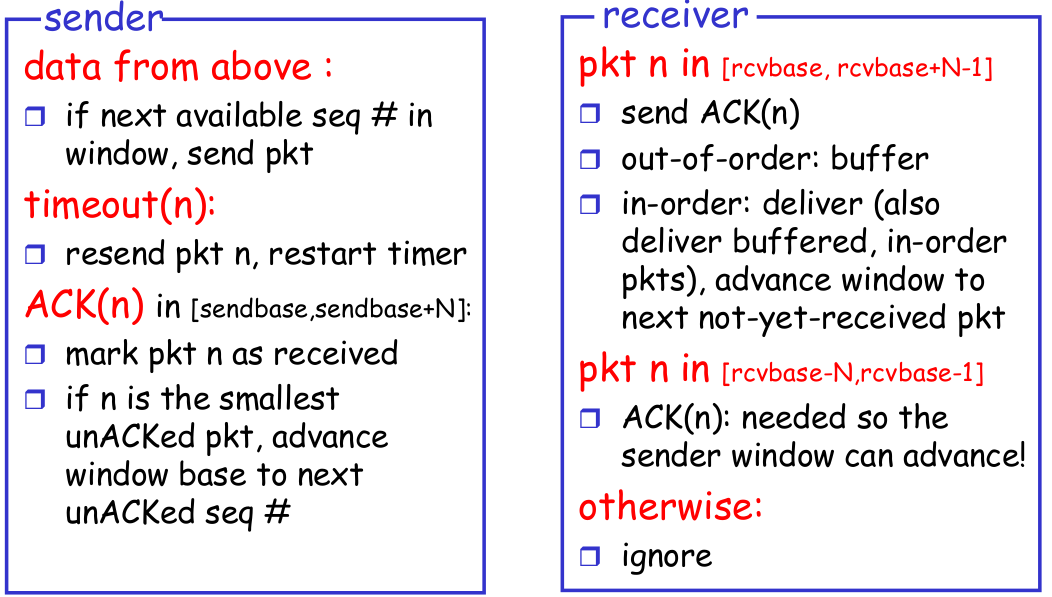
\includegraphics[width=0.48\textwidth]{sr}
\end{figure}

\subsection{Connection-oriented transport: TCP}

\key{TCP segment structure}
\begin{figure}[H]
  \centering
  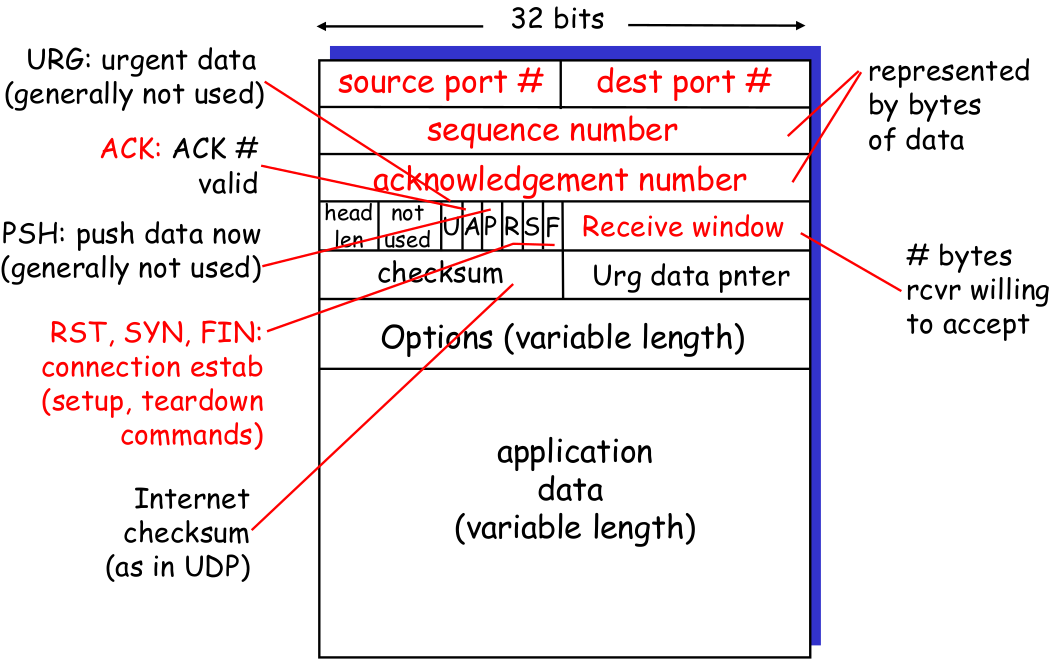
\includegraphics[width=0.48\textwidth]{tcp_frame}
  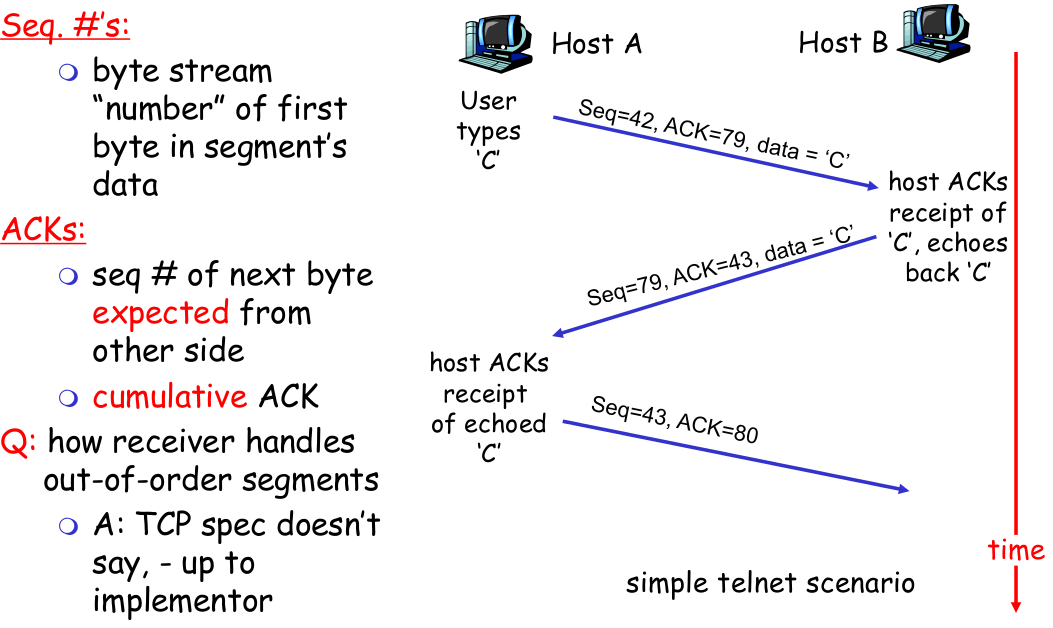
\includegraphics[width=0.48\textwidth]{tcp_seq}
\end{figure}

\key{TCP Connection Establishment (3-way) and Close}
\begin{figure}[H]
  \centering
  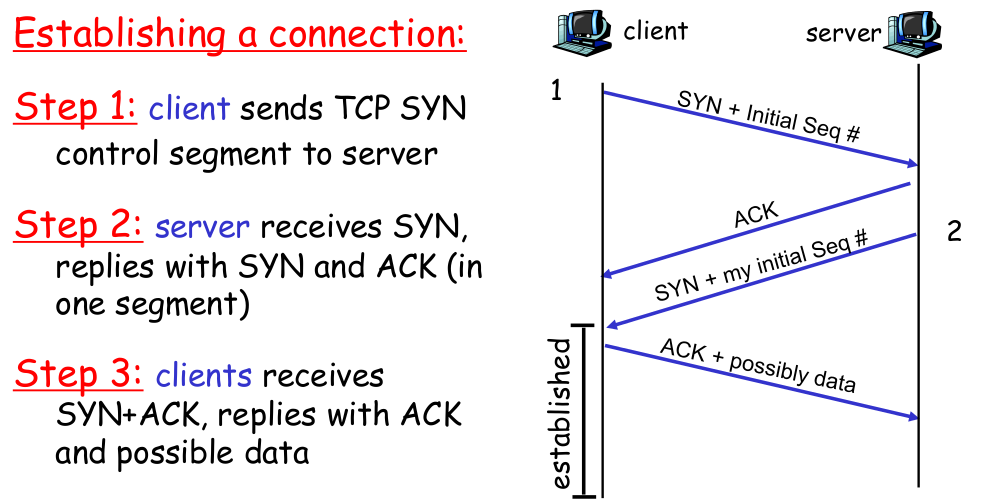
\includegraphics[width=0.48\textwidth]{tcp_conn}
  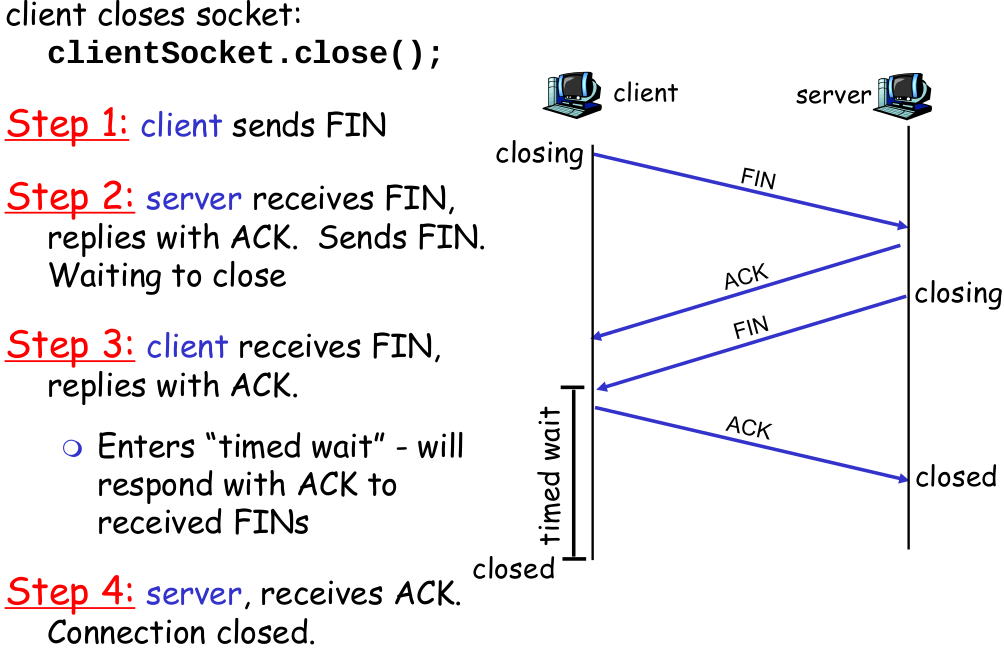
\includegraphics[width=0.48\textwidth]{tcp_close}
\end{figure}

\subsection{TCP congestion control}

\key{Congestion} Too many sources sending too much data too fast for network to handle

\key{TCP AIMD}
\begin{figure}[H]
  \centering
  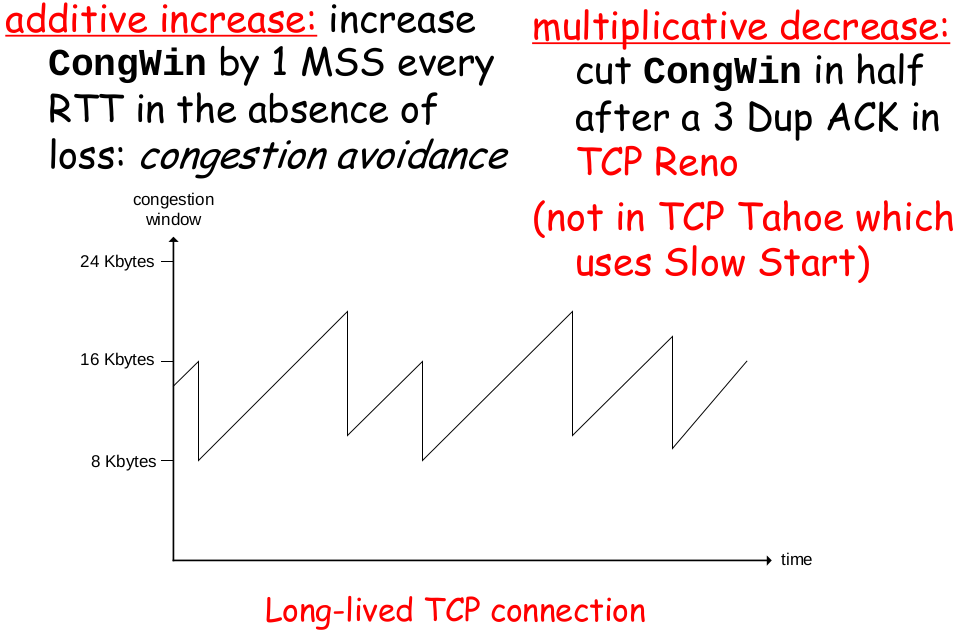
\includegraphics[width=0.5\textwidth]{tcp_aimd}
\end{figure}

\key{Fast Retransmit (Reno)}
\begin{figure}[H]
  \centering
  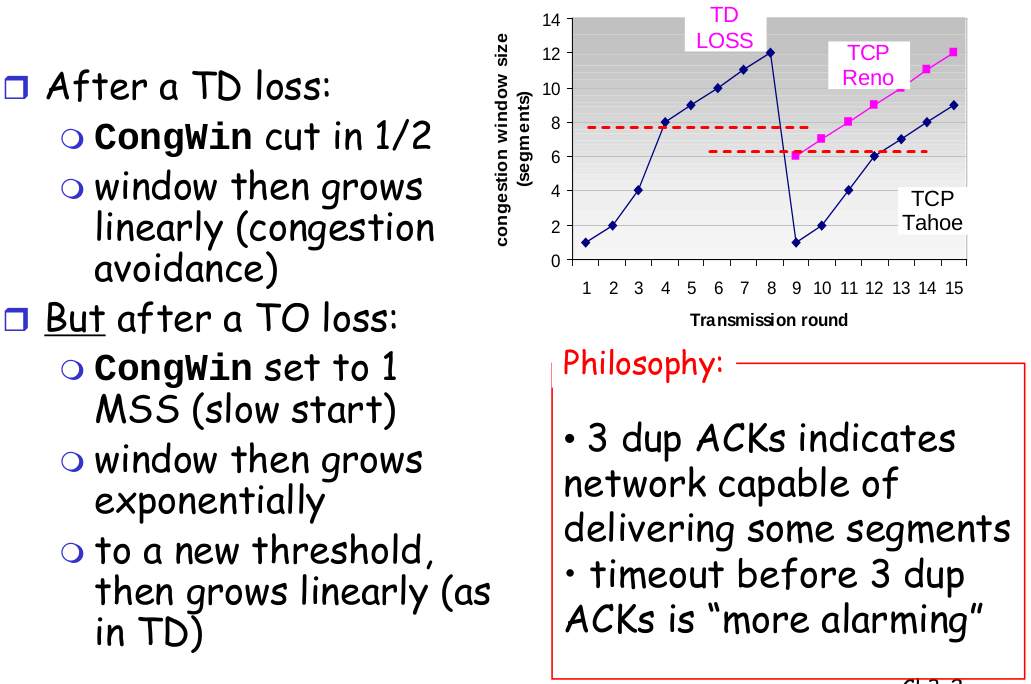
\includegraphics[width=0.48\textwidth]{tcp_reno}
  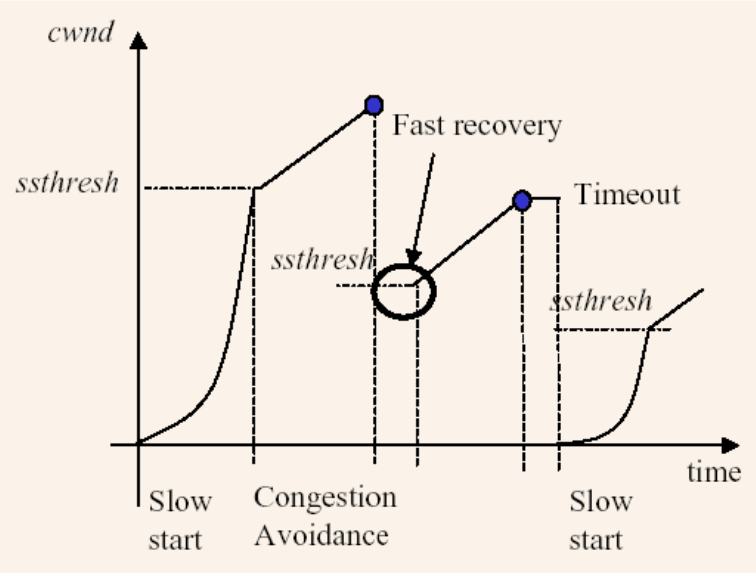
\includegraphics[width=0.48\textwidth]{tcp_phase}
\end{figure}

\key{Why is TCP fair?}
\begin{figure}[H]
  \centering
  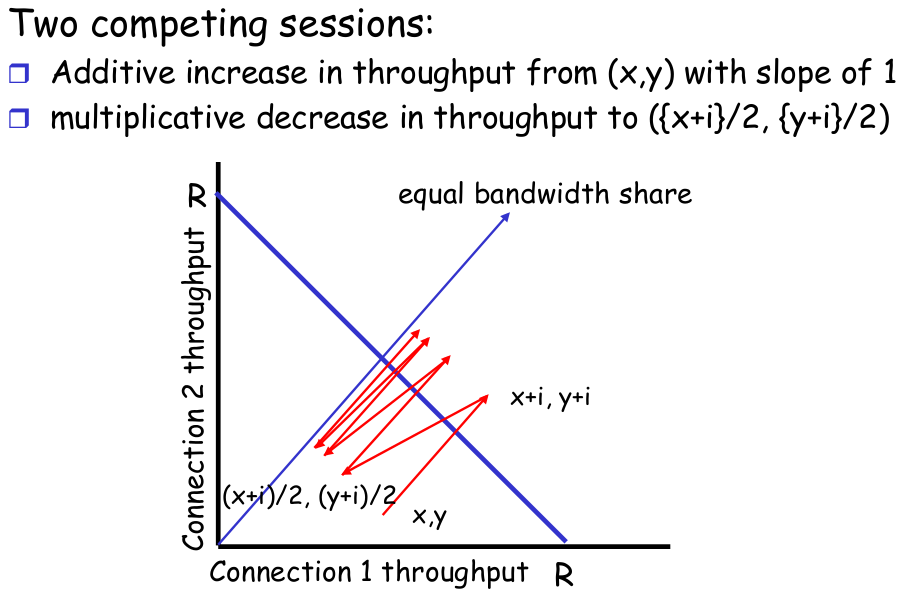
\includegraphics[width=0.5\textwidth]{tcp_fair}
\end{figure}

\key{TCP Delay}
$R$ link rate, $S$ MSS size, $O$ object/file size, $W$ window size
\begin{figure}[H]
  \centering
  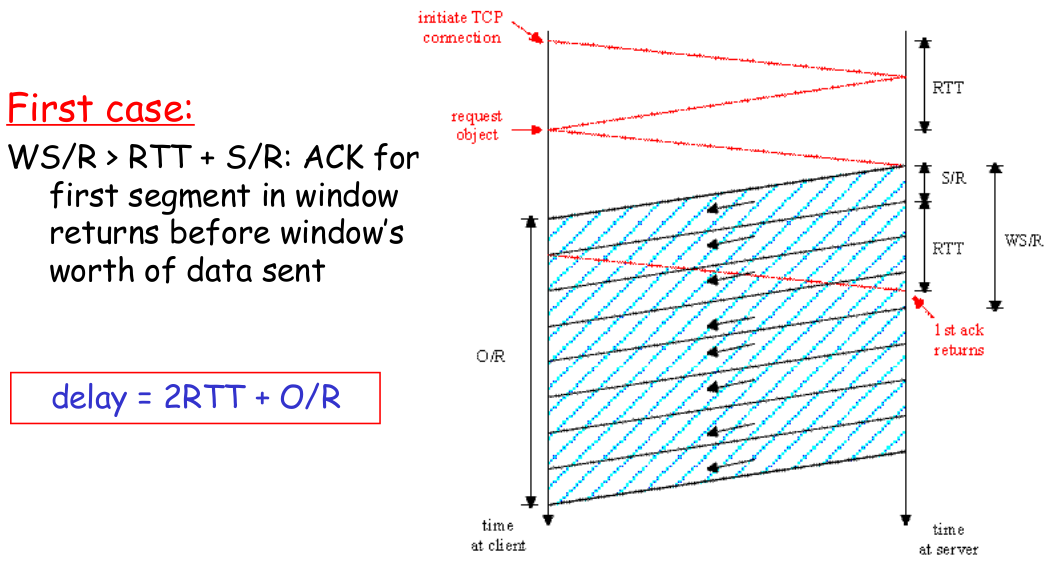
\includegraphics[width=0.48\textwidth]{tcp_delay1}
  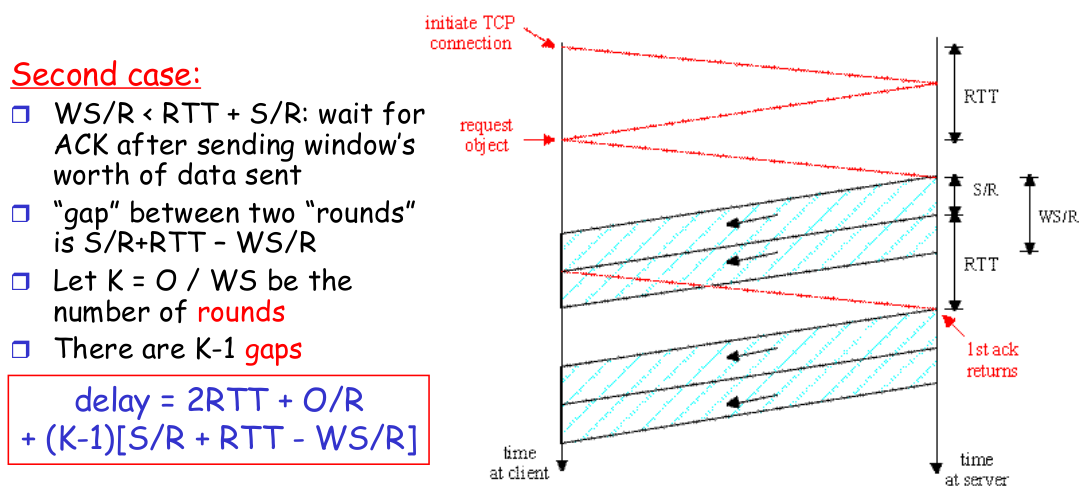
\includegraphics[width=0.48\textwidth]{tcp_delay2}
\end{figure}
